%\documentclass[11pt]{article}
\documentclass{asme2ej}
\usepackage{amsmath,amssymb,graphicx,bm}
\usepackage{listings, xcolor, subcaption, placeins}
\usepackage{undertilde}
\usepackage{algorithm,algpseudocode}
\usepackage{multicol}
\usepackage{makecell}
\usepackage[table]{colortbl}
%%%%%%%%%%%%%%%%%%%%%%%%%%%%%%
%%%%%%%%%%%%%%%%%%%%%%%%%%%%%%
%%%%%%%%%%%%%%%%%%%%%%%%%%%%%%

%% If you want to define a new command, you can do it like this:
\newcommand{\Q}{\mathbb{Q}}
\newcommand{\R}{\mathbb{R}}
\newcommand{\Z}{\mathbb{Z}}
\newcommand{\C}{\mathbb{C}}
\newcommand{\e}{\bm{e}}
\newcommand{\TEN}[1]{\underline{\underline{#1}}}
\newcommand{\TOT}[1]{\underline{\underline{\underline{#1}}}}
\newcommand{\VEC}[1]{\utilde{#1}}
\newcommand{\UVEC}[1]{\underline{#1}}
\newcommand{\PK}[1]{\TEN{\tau}^{(#1)}}
\newcommand{\cauchy}{\TEN{\sigma}}
\newcommand{\st}{$^{\text{st}}$}
\newcommand{\nd}{$^{\text{nd}}$}
\newcommand\defeq{\mathrel{\stackrel{\makebox[0pt]{\mbox{\normalfont\tiny def}}}{=}}}
\newcommand{\micro}[1]{{#1}'}
\newcommand{\GDNSDOF}{$\left\{\breve{Q}\right\}$}
\newcommand{\GMMCDOF}{$\left\{\breve{D}\right\}$}

\graphicspath{{./img/}}

%% If you want to use a function like ''sin'' or ''cos'', you can do it like this
%% (we probably won't have much use for this)
% \DeclareMathOperator{\sin}{sin}   %% just an example (it's already defined)


\begin{document}
\title{Overlap Coupling Implementation}
\author{Nathan Miller}

\maketitle

\begin{abstract}
The documentation for the overlap coupling is presented. This documentation details the theoretical background of the implementation along with the implementation into code. Documentation which also communicates the method by which the coupling is joined into the simulation tool Abaqus using the SIMULIA Co-Simulation Engine (CSE) is also detailed.
\end{abstract}

\section{Nomenclature}

\begin{table}[htb!]
\centering
\begin{tabular}{|c|l|}
\hline
$x_i$ & Position of the center of mass of the differential element in the\\
& current configuration\\
\hline
$X_I$ & Position of the center of mass of the differential element in the\\
& reference configuration\\
\hline
$\xi_I$ & Position of the center of mass of the micro element in the\\
& current configuration w.r.t. the center of mass of the differential element\\
\hline
$\Xi_I$ & Position of the center of mass of the micro element in the\\
& reference configuration w.r.t. the center of mass of the differential element\\
\hline
$\sigma_{ij}$ & Unsymmetric Cauchy stress\\
\hline
$s_{ij}$ & Symmetric micro stress\\
\hline
$m_{ijk}$ & Higher order couple stress\\
\hline
$f_{i}$ & Body force density\\
\hline
$a_{i}$ & Acceleration\\
\hline
$l_{ij}$ & Body force couple\\
\hline
$\omega_{ij}$ & Micro-spin inertia\\
\hline
$\tilde{\mathcal{B}}^h$ & The free micromorphic finite element overlap with ghost DNS domain\\
\hline
$\overline{\mathcal{B}}^h$ & The pure micromorphic domain\\
\hline
$\hat{\mathcal{B}}^h$ & The ghost micromorphic finite element overlap with free DNS domain\\
\hline
$\overline{\mathcal{B}}^{DNS}$ & The pure DNS domain\\
\hline
\GDNSDOF & The generalized DNS DOF vector\\
\hline
\GMMCDOF & The generalized micromorphic DOF vector\\
\hline
$\left\{\hat{Q}\right\}$ & The DNS DOF prescribed by micromorphic fields $\left(\alpha \in \hat{\mathcal{A}} \in \tilde{\mathcal{B}}^h\right)$\\
\hline
$\left\{\hat{D}\right\}$ & The nodes of the micromorphic continuum overlapping the DNS $\left(a \in \hat{\mathcal{N}}\ f \in \hat{\mathcal{M}}\quad \hat{\mathcal{N}},\hat{\mathcal{M}} \in \tilde{\mathcal{B}}^h \cup \hat{\mathcal{B}}^h\right)$\\
\hline
$\left\{D\right\}$ & The free DNS nodes $\left(m \in \mathcal{N}\ n \in \mathcal{M}\quad \mathcal{N},\mathcal{M} \in \tilde{\mathcal{B}}^h \cup \overline{\mathcal{B}}^h\right)$\\
\hline
$\VEC{q}_{\alpha}$  & The positional DOF vector for DNS  node $\alpha$ $\left(\alpha,\ \beta,\ldots \in \breve{\mathcal{A}}\right)$\\
\hline
$\VEC{d}_a$ & The macro-position vector for micromorphic node $a$ $\left(a,b,\ldots \in \breve{\mathcal{N}}\right)$\\
\hline
$\left\{\phi\right\}_f$ & The micro-dof vector for micromorphic node $f$ $\left(f,g,\ldots \in \breve{\mathcal{M}}\right)$\\
\hline
\end{tabular}
\end{table}

\FloatBarrier

\section{Introduction}

One of the most powerful (and exciting) applications of the micromorphic continuum theory is in the development of an overlap coupling between regions of low fidelity which are modeled using the micromorphic continuum and regions of high fidelity which model the microstructural response directly. In this way, models can be developed which both can efficiently solve problems via using high fidelity representations of the material only in the regions where this is absolutely necessary. The Micromorphic continuum can be used in other regions where this assumption is accurate enough.

Importantly, the communication between length scales is bi-directional in that neither the DNS nor the continuum representation are exclusively driven by the other. Rather, the information is communicated between the two using an overlap coupling scheme as developed by \cite{bib:klein06}. We now describe the theoretical background for the coupling process.

\section{Degree of Freedom Coupling}

The coupling between the degrees of freedom in the micromorphic and DNS domains is shown in Figure~\ref{fig:overlapping_domains}. As can be seen, the DNS can either be interacting with the micromorphic continuum or a standard continuum. The full micromorphic domain can be written as $\overline{\mathcal{B}}^h \cup \hat{\mathcal{B}}^h \cup \tilde{\mathcal{B}}^h$. Our primary goal is to reduce the size of the DNS domain $\overline{\mathcal{B}}^h$ and still retain the macro-response. In this way we will reduce the cost of a simulation which, in general, could be intractable to one which can be solved in a reasonable amount of computational time.

\begin{figure}[htb!]
\centering
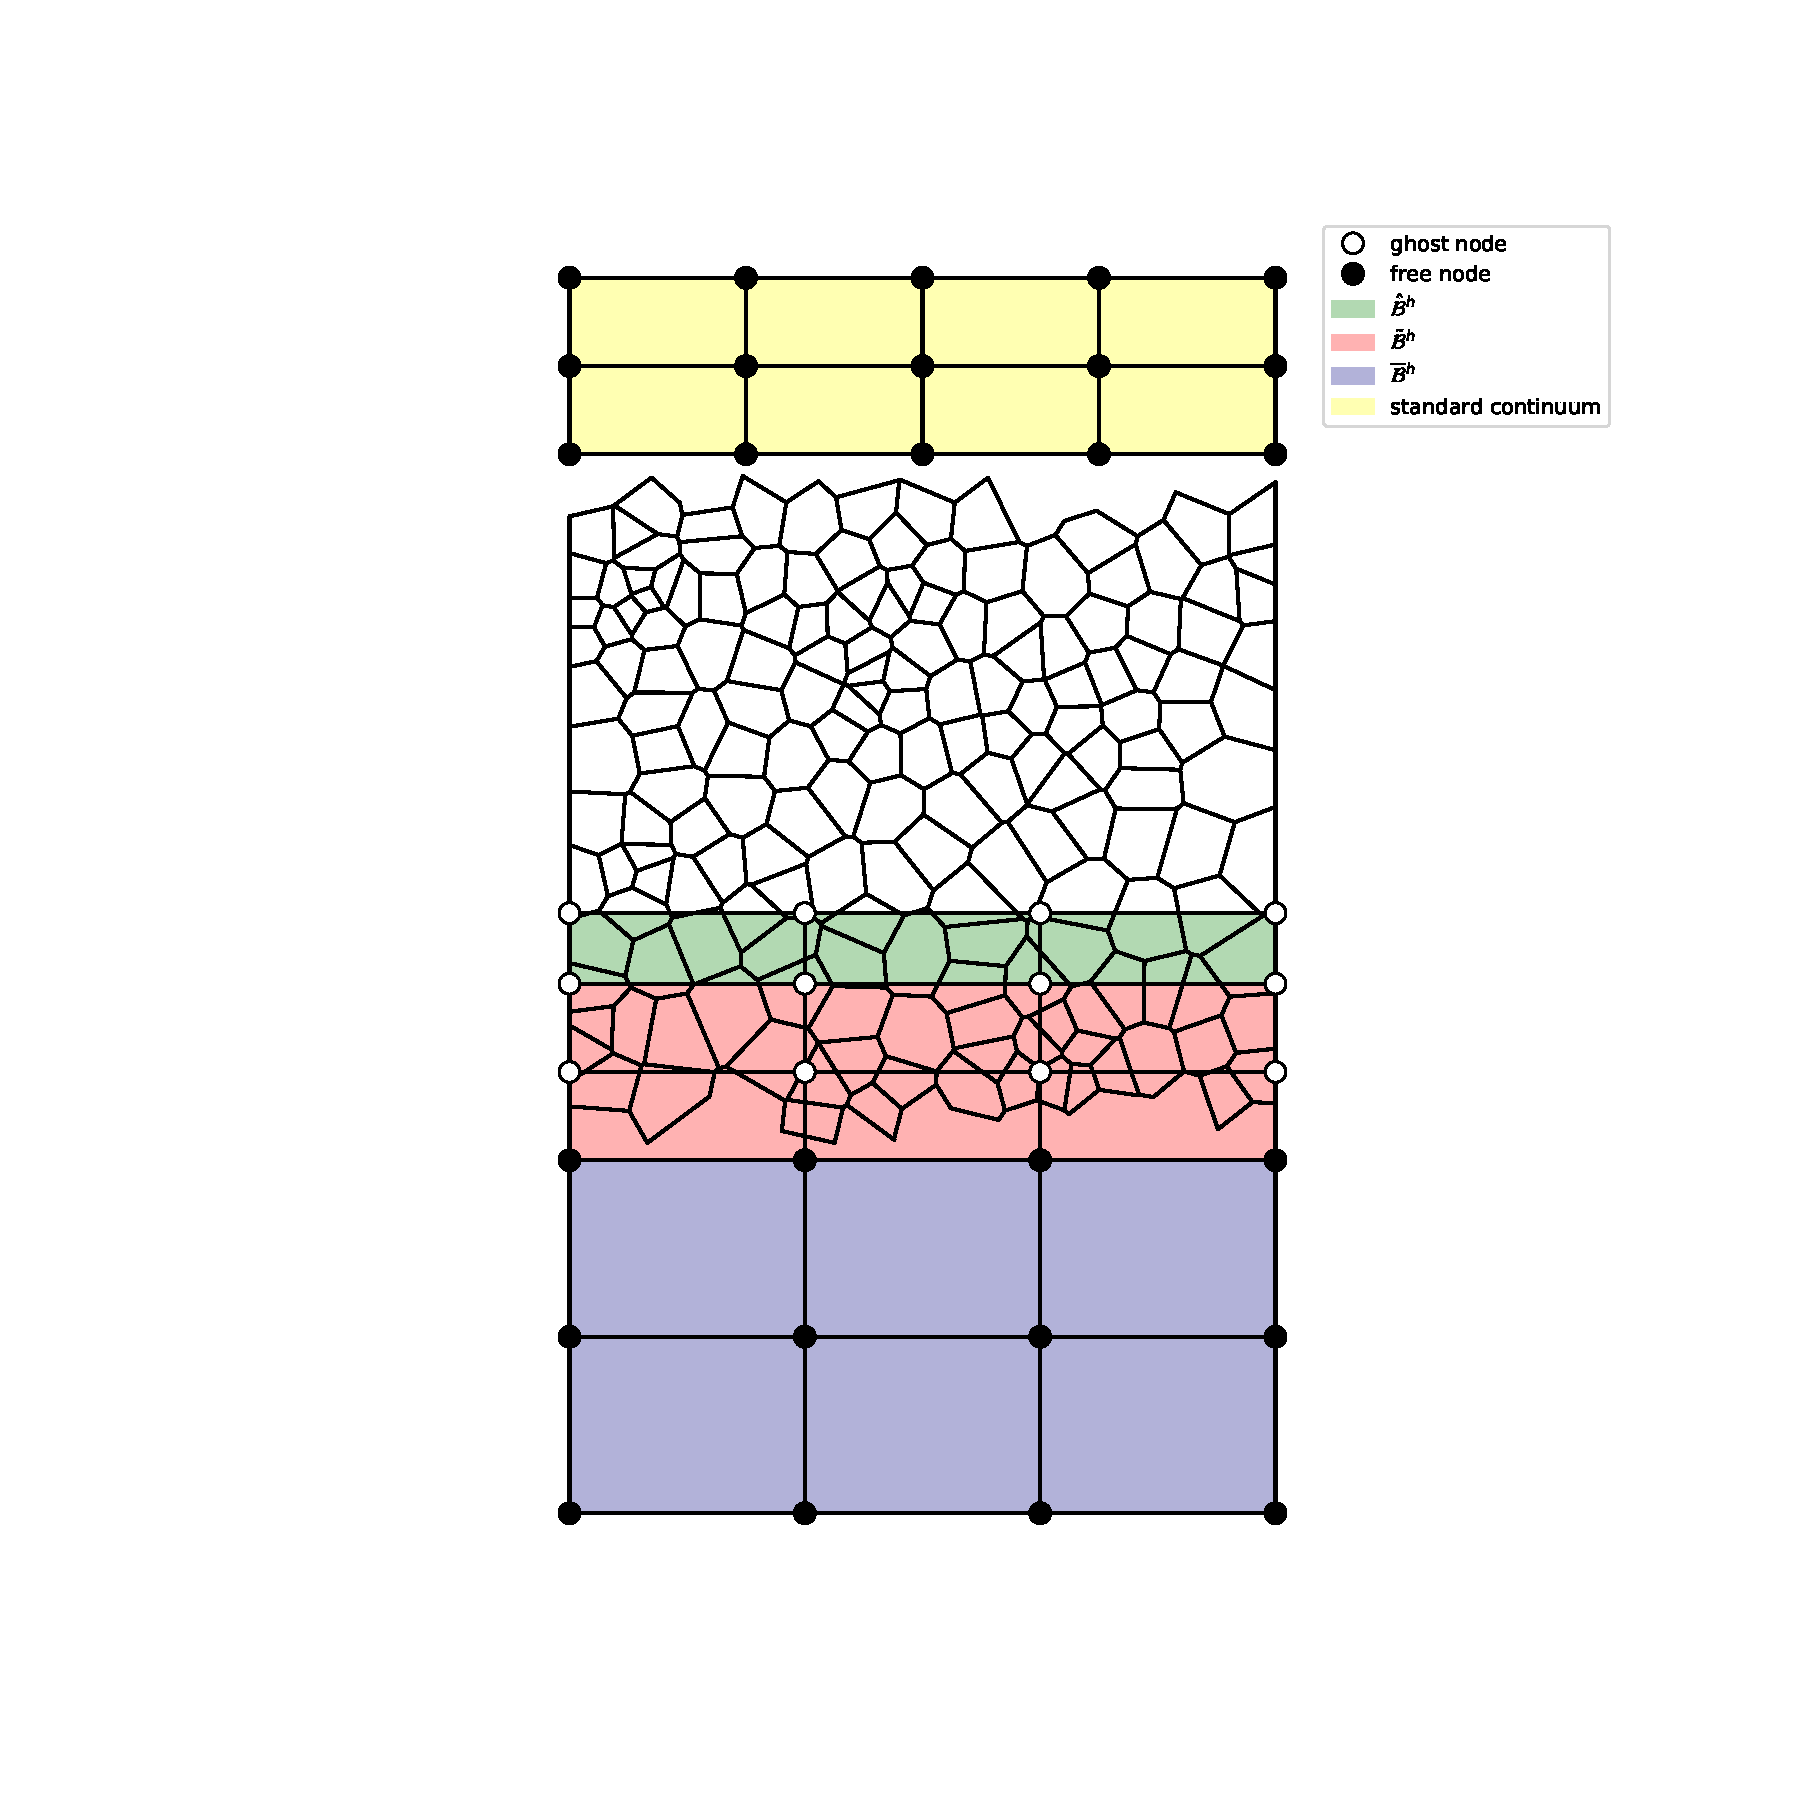
\includegraphics[width=0.7\textwidth]{overlapping_domains.pdf}
\caption{Schematic of overlapping domains}
\label{fig:overlapping_domains}
\end{figure}

We interpolate the micromorphic finite element to the DNS DOF to provide boundary conditions on the DNS in the reference configuration by recognizing that the macro and micro degree of freedom vectors at macro DOF node $a$ and micro DOF node $b$ can be mapped to the DNS point via
\begin{align*}
\VEC{u}_{\alpha} &= \sum_{a \in \breve{\mathcal{N}}} N_a^{u,e} \left(\VEC{X}_{\alpha}^h\right) \VEC{d}_a^e(t)\\
\left\{\phi\right\}^e_{\alpha} &= \sum_{b \in \breve{\mathcal{M}}} N_b^{\phi,e} \left(\VEC{X}_\alpha\right) \left\{\phi\right\}_b^e(t)\\
\end{align*}

for all $\alpha \in \breve{\mathcal{A}}$. We note that for any point in the DNS $\alpha$ we can also write with respect to the center of mass of the associated micromorphic element $e$
\begin{align*}
\left(\micro{\VEC{x}}\right)_{\alpha}^e &= \VEC{x}^e + \VEC{\xi}_{\alpha}^e
\end{align*}

where $\VEC{x}^e$ is the global position of the center of mass of $e$ and $\VEC{\xi}_{\alpha}^e$ is the location of the DNS node $\alpha$ with respect to $\VEC{x}^e$. We also note that we can write
\begin{align*}
\VEC{x}^e &= \VEC{X}^e + \VEC{u}^e\\
\VEC{\xi}_{\alpha}^e &= \TEN{\chi}_{\alpha}^e \cdot \VEC{\Xi}_{\alpha}^e = \left(\TEN{I} + \TEN{\phi}_{\alpha}^e\right) \cdot \VEC{\Xi}_{\alpha}^e\\
\end{align*}

where $\TEN{\phi}_{\alpha}^e$ is found by reconstructing $\left\{\phi\right\}_{\alpha}^e$ into tensor form. By asserting that we can write
\begin{align*}
\left(\micro{\VEC{x}}\right)_{\alpha}^e &\defeq \left(\micro{\VEC{X}}\right)_{\alpha}^e + \left(\micro{\VEC{u}}\right)_{\alpha}^e\\
\end{align*}

where $\left(\micro{\VEC{u}}\right)_{\alpha}^e$ is defined as a micro-displacement vector we can write
\begin{align*}
\left(\micro{\VEC{x}}\right)_{\alpha}^e &= \left(\micro{\VEC{X}}\right)_{\alpha}^e + \left(\micro{\VEC{u}}\right)_{\alpha}^e\\
\end{align*}

\section{Coupling Scheme}

\FloatBarrier

\bibliographystyle{asme2ej}
\bibliography{micromorphic}

\end{document}